\documentclass[11pt]{article}
\usepackage{../EllioStyle}

\title{Homework 3}
\author{Elliott Pryor \\
Collaborated with: Nathan Stouffer}
\date{09 March 2021}

\rhead{Homework 3}
\lhead{Elliott Pryor}

\graphicspath{{./}{images/}}




\makeatletter
\def\mathcolor#1#{\@mathcolor{#1}}
\def\@mathcolor#1#2#3{%
  \protect\leavevmode
  \begingroup
    \color#1{#2}#3%
  \endgroup
}
\makeatother


\algdef{SE}[DOWHILE]{Do}{doWhile}{\algorithmicdo}[1]{\algorithmicwhile\ #1}

\begin{document}

\maketitle

\problem{1}

Given an polygonal chain $P$ of $n$ vertices, we define an vertex $v$ as a
\emph{local max} if $v$ if all edges adjacent to $v$ are to the left of $v$.
Show that can determine if a polygonal chain with $k$ local maxes is simple in
$O(n \log k)$ time.

\hrule







\problem{2}

A friend of yours from the civil engineering department wants to analyze whether
a dangerous portion of a river will flood. He presents you with the following
(admittedly rather unrealistic) model of the river. The portion of the river of
interest is modeled as an $x$-monotone polygon $P$ that is bounded between two
vertical lines at $x = x^-$ and $x = x^+$ (see Figure). The river is bounded on
its left and right ends by two vertical line segments of lengths $w^-$ and
$w^+$, respectively. Inside the polygon are some number of disjoint x-monotone
polygons that represent islands in the river.  Let $n$ denote the total number
of vertices, including both the outer banks of the river and the islands.

\begin{figure}[h]
    \centering
    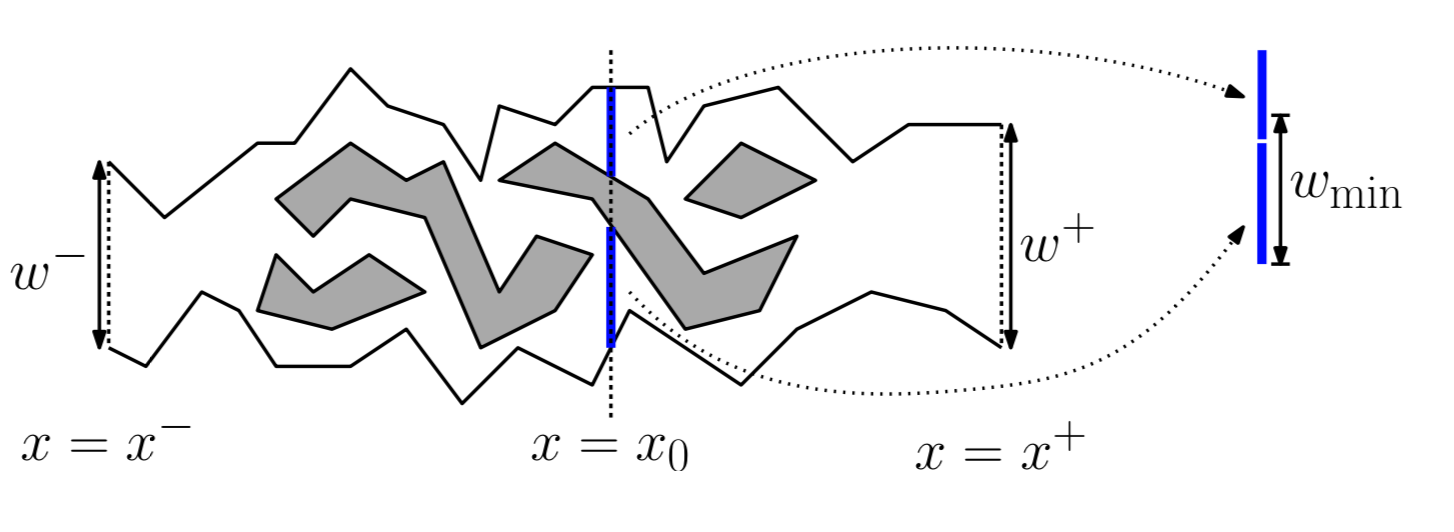
\includegraphics[width=0.75\textwidth]{river}
    \caption{Problem 2: River}
\end{figure}

Your friend tells you that the in order to avoid a flood, the width of the river
(not counting islands) at every vertical cut must be at least some minimum value
$w_{min}$. For example, in the figure, the sum of the two blue vertical segments
at $x = x_0$ must be at least $w_{min}$ in order to avoid a flood.  Given the
polygon $P$ and the value $w_{min}$, present an $O(n \log n)$ time algorithm that
determines whether the river will flood, that is, whether there is a vertical
cut whose total width is smaller than $w_{min}$. If it will flood, your algorithm
should output the value $x_0$ of the bottleneck, that is, the location where the
sum of vertical lengths (excluding islands) is the smallest.

\begin{enumerate}

    \item Hint 1: There is an (uncountably) infinite number of possible vertical
        cuts to consider. Prove that it suffices to check the width at a
        discrete set of locations, whose number is $O(n)$.

    \item Hint 2: There is a bit of a trick to updating the vertical widths
        (excluding the islands). For partial credit, explain how to do it under
        the assumption that the sweep line can only intersect a constant number
        of islands at any time. (For example, in the figure, the sweep line
        never hits more than two islands at a time.) For full credit, explain
        how to do it even if the number of islands hit by the sweep line at any
        time could be as high as $\Omega(n)$.
\end{enumerate}
\hrule


So we first create a list of the event points. An event point stores an $x$ location,
and a pointer to a vertex. We create one event point per vertex. 
Each event point will also have the slope of the `left' edge
and the slope of the `right' edge.
One of these are 0 if the vertex is leftmost or rightmost in polygon (e.left = 0 if e is leftmost point).
Then we have a sign value (s) which is $-1$ or $1$ if the vertex is on upper hull or lower hull respectively.
(One small technicality that the river bank is labeled with opposite sign (ie e.s of a vertex on upper bank of river is $+1$ instead of $-1$))


We then sort the event points by $x$ coordinate. 

On the sweepline we will store 2 variables: $a, b$ that will define our width function. 

We iterate over the events. For each event we set $a = f(e)$, and $b = b + e.s (e.right - e.left)$.
Our function $f$ is evaluated as $f(e) = a + b (e.x - e_{-1}.x)$ where 
$(e.x - e_{-1}.x)$ denotes the distance between this point and the previous event point.

We then have a global variable storing the minimum value of $a$.

\begin{algorithm}
    \caption{Flood!!!}
    \label{alg:neighbors}
    \begin{algorithmic}[1]
    \Function{flood}{$B, P[]$}
        \State initialize events
        \State sort events by $x$
        \State $min \gets +\infty$
        \State $a \gets w^-$, $b \gets 0$
        \For{$e \in events$}
            \State $a \gets f(e)$
            \State $min \gets a$ if $a < min$
            \State $b \gets b + e.s (e.right - e.left)$
        \EndFor
        \State \textbf{return} min
    \EndFunction
    \end{algorithmic}
\end{algorithm}

\textbf{Runtime:} Initialize events takes $O(n)$ since it is done with a single linear pass through events and constant time operations.
Sorting takes $O(n \log n)$. The internal operations of the for loop are $O(1)$. 
It runs over each event so there are $O(n)$ operations in the for loop.

Thus in total: $O(n \log n)$


\textbf{Correctness:} 
This hinges on the correctness that our function $f$ correctly evaluates the width at a point.
\newpage
\begin{proof}
    By Induction.

    Base case is at the leftmost point. We initialize $a = w^-$ and $b = 0$, so $f = w^-$
    at the leftmost point. We then show that it correctly computes the width at the next point.
    We assume that there are no islands at the beginning, so it just needs to compute the width
    of the channel. The rate of change in channel width is the slope of upper bank - slope of lower bank
    Thus we have in our algorithm: $b \gets 0 + (1) (u.right - 0) + (-1)(l.right - 0) = u.right - l.right$
    where $u$ is the event of upper bank, and $l$ is lower bank. This is the same as what we described
    intuitively above. Therefore the base case holds and the function describes the width at the next event point.

    Inductive step: assume that the function correctly computes the width up to this event point.
    Show that it correctly computes at the next event point.

    We have two cases: the first case is that this event point is not the start of an island. The second case is the event is the start of an island.
    
    Case 1: So we examine how the rate of change changes. It is not changing anywhere else except at the event point.
    So we need to analyze the change at the point.
    It is no longer changing by the rate of the left side so
    we subtract $e.s * e.left$, and now if it is on the top of a polygon (island), it is changing by $(-1) * e.right$
    since a positive slope means the channel is contracting. And on the bottom it is now changing by $(1) * e.right$.
    This is just the sign $e.s$, so we add $e.s * e.right$, or $e.s * e.right - e.s *e.left = e.s(e.right - e.left)$.
    Thus our rate of change update is correct and it correctly measures the width at the next event point.

    Case 2: It is the beginning of an island. Then we just need to subtract off the wedge that is formed by the start of the island.
    We split it up into 2 events $u, l$ where $u$ is the upper slope and $l$ is the lower slope. 
    So $u.right > 0$ and $l.right < 0$. So we want to add $l.right$ and subtract $u.right$. So 
    $b \gets b - u.right + l.right = b + (-1) (u.right - 0) + (1) (l.right - 0) = b + u.s (u.right - u.left) + l.s (l.right - l.left)$.
    Since addition is associative we can do these events separately.
    Thus, our rate of change of the width is still correct and we correctly evaluate the width at the next point.

    So in both cases the rate of change is correct. Then the width at the next point is as follows.
    width at this point + rate of change * change in x. Well that is $f(next \: e) = a + b * (next \: e_x - e_x)$.
    Which must be the width at the next point, otherwise the change in width is not described by $b * (next \: e_x - e_x)$,
    a contradiction since $b$ correctly describes the rate of change of width.

\end{proof}



\problem{3}

\begin{enumerate}

    \item (7 points) Describe and analyze an algorithm that computes the
        convex hull of a set of $n$ points in the plane using randomized
        incremental construction in expected $O(n \log n)$ time. For this
        problem you are welcome to find an algorithm and its analysis on the
        web, but please cite where you found it, describe it concisely in
        your own words, and make the analysis very concise. Where does the
        log-factor come from?

    \item (3 points) Give an example of a set of points in the plane, and a
        particular input order, that causes the convex hull algorithm to run in
        $O(n^2)$ when the points are added in this particular order. Make sure it
        is clear how your example generalizes to arbitrary values of $n$.

\end{enumerate}
\hrule

\subsection*{1. }

\begin{figure}[h]
    \centering
    \begin{subfigure}{0.7 \textwidth}
        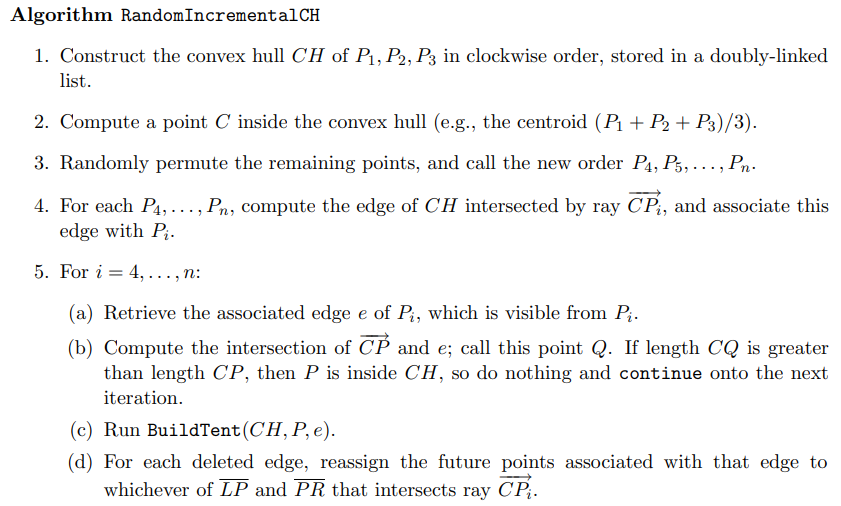
\includegraphics[width = \textwidth]{randomized_CH.png}
        \caption{Randomized Convex Hull algorithm}
    \end{subfigure}
    \begin{subfigure}{0.7 \textwidth}
        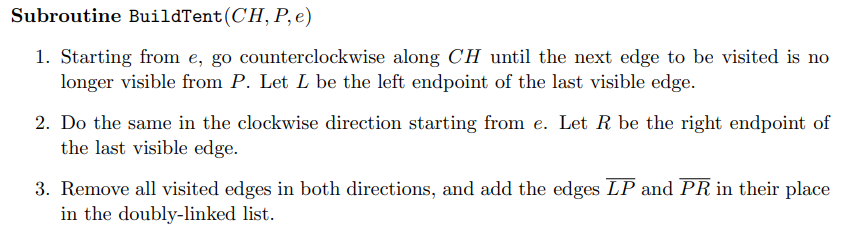
\includegraphics[width = \textwidth]{buildTent.png}
        \caption{Subroutine `build tent' that detects what edges to replace}
    \end{subfigure}
    \caption{Randomized convex hull algorithm taken from 
    \href{http://www.cs.cmu.edu/afs/cs/academic/class/15750-s17/ScribeNotes/Lecture15/lecture15.pdf}{Lecture 15 of 15-750 Graduate Algorithms at Carnegie Mellon University}}
\end{figure}

Above is the description copied from Carnegie Mellon University lecture notes.

\textbf{Alg}
We start by initializing the convex hull to be 3 random points from the point set.
They then find some point in the interior of the convex hull: the centroid $C = \frac{P_1 + P_2 + P_3}{3}$.
(the middle of the convex hull).

Then considering a random permutation of the points, they compute an edge that is `visible' to $P_i$.
An edge is associated with $P_i$ if ray $C, P_i$ intersects the edge. 
Then, we build the convex hull:

For each point, get the edge that is visible to it. Then check if the point is within the convex hull.
Let $Q$ be the point where the ray $C, P_i$ intersects the visible edge. The point is inside iff $dist(C, P_i) < dist(C, Q)$.
If $P_i$ is inside, then we don't need to do anything: move on.

If $P_i$ is outside, then we run BuildTent, to compute the left and right vertices. 
These are the vertices that are tangent to $P_i$. 
They then delete the edges between $L, R$ and replace them with $L,P_i$ and $P_i, R$.
Then the points that were associated with deleted edges get re-assigned to either 
$L,P_i$ or $P_i, R$ based on the ray intersection from the initialization.

\textbf{Runtime: }
Step 1, takes $O(1)$ since we make a convex hull of fixed size 3.
Step 2, takes $O(1)$ since we compute the centroid.
Step 3, takes $O(n)$ since we shuffle all the points. 
Step 4, takes $O(n)$, this is a little bit less trivial. But we know that we can check
line intersections in $O(1)$. We then consider an edge in the convex hull, we can iterate through
the entire list of points and check if the ray intersects the line segment in constant time. So this takes $O(n)$.
We then only have 3 edges to consider, so $O(n)$ in total.
So the entire initialization routine goes $O(n)$

Then we use backwards analysis. We remove a random point $P_i$ from the convex hull,
and analyze the cost of doing so. When we remove a point from the CH we must pay a cost of `undoing' the BuildTent operation.
So we pay a cost related to the number of points whose ray intersects these two edges.
For each point $q$ outside the CH, ray $C,q$ intersects one edge, which is defined by 2 vertices.
So the probability that we pay the cost of $q$ by removing $P_i$ is the probability $P_i$ is one
of these 2 vertices: or $2/|CH|$. There are at most $n-i$ vertices on the CH (every vertex that we haven't removed)
and $i$ points outside the CH. So summing over all $i$ we get:
$\sum_{i = 0} ^n i \cdot 2/(n-i)$. We do change of variables $j = n-i$ (intuitively $j$ is number of vertices on the CH)
$$\sum_{i = 0} ^n i \cdot 2/(n-i) = \sum_{j = 0} ^n (n-j) \cdot 2/j \leq \sum_{j = 0} ^n (n) \cdot 2/j = 2n \cdot \sum_{j = 0} ^n 1/j = 2n \Theta(\ln n) = O(n \log n)$$

The log factor comes from the harmonic series. But physically it comes from the probability that we have to update what edge a point is associated with.

\subsection*{2. }

So we get $O(n^2)$ if we have to update what edge a point is associated with every single time
for every point. 

Consider the points $(0,0), (-1, -1)$ then $p_n = (n, 1/n)$ for $n \geq 1$.
If our initial 3 points are $(0,0),(-1,-1),(1,1)$ then every point is associated with
edge $[(1,1), (-1,1)]$. Then when we update every point $p_j$ is then associated with $[(n,1/n), (-1,1)]$
for $j > n$, and all the points $j \leq n$ are inside the convex hull. 


\begin{figure}[h]
    \centering
    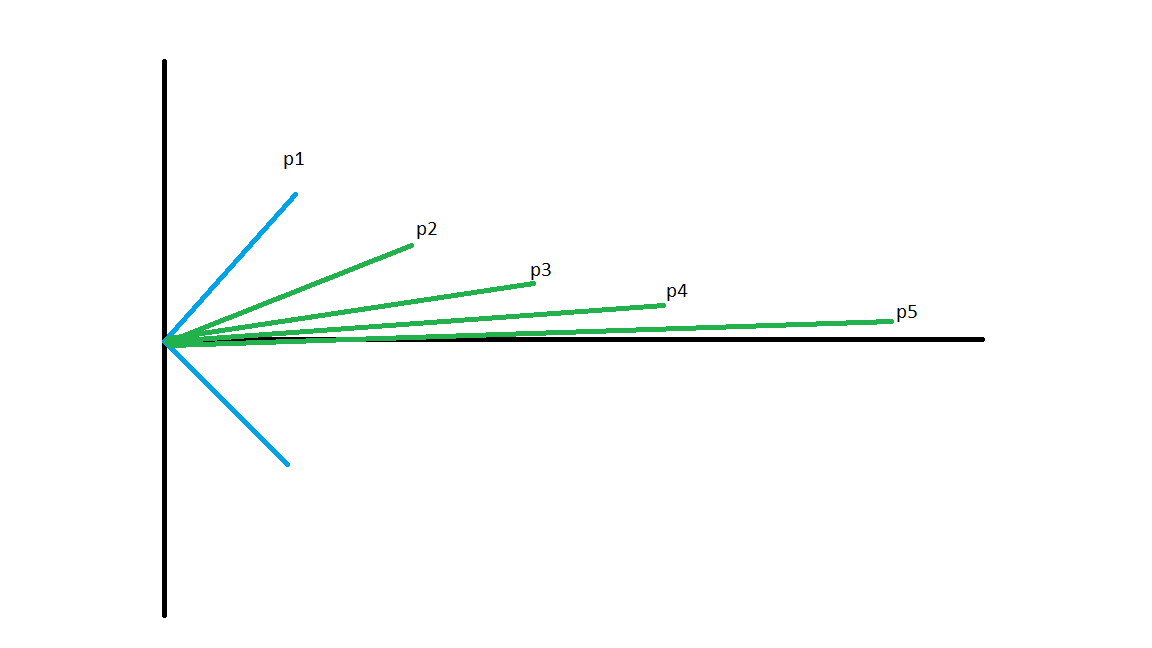
\includegraphics[width=0.5\textwidth]{bad}
    \caption{Showing the points and rays resulting in $O(n^2)$}
\end{figure}













\problem{4}

Consider the following instance of the trapezoidal map point location data
structure. The left side shows the map, and the right side shows the
corresponding DAG. Describe the resulting trapezoidal map and DAG after segment
$xy$ has been added.

\begin{figure}[h]
    \centering
    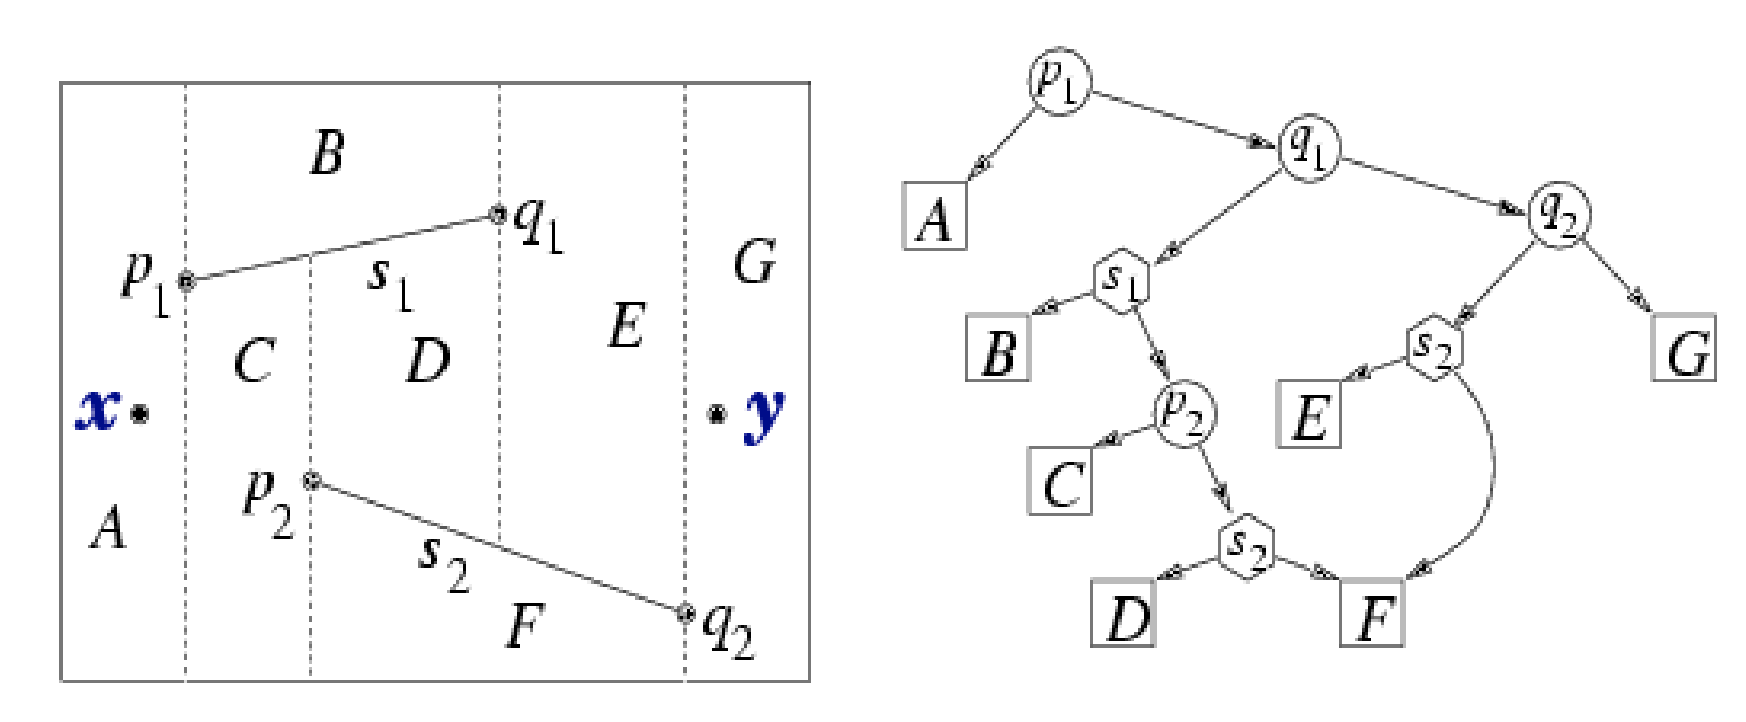
\includegraphics[width=0.75\textwidth]{trapMap}
    \caption{Problem 4: Trapezoid Map}
\end{figure}
\hrule


\begin{figure}[h]
    \centering
    \begin{subfigure}{0.3 \textwidth}
        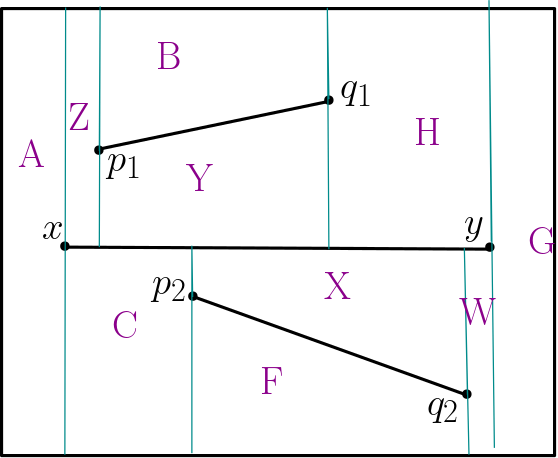
\includegraphics[width = \textwidth]{traps}
        \caption{Trap map after adding segment xy}
    \end{subfigure}
    \begin{subfigure}{0.65 \textwidth}
        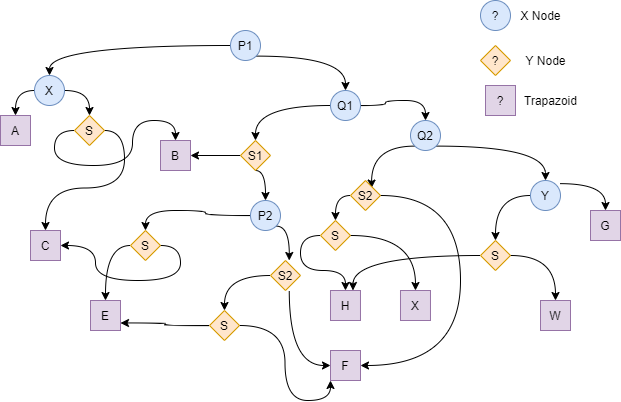
\includegraphics[width = \textwidth]{Tree}
        \caption{DAG after adding line segment xy}
    \end{subfigure}
    \caption{DAG and Tree resulting from adding segment xy}
\end{figure}


So the DAG became a bit of a tangled mess. I apologize. 

Essentially we just add vertical lines from $x$ and $y$. 
Then we trim the lines that we intersect with the horizontal line segment.
Then in order to build the tree. We take the original map, and apply the 3 cases to it,
although we only need cases 1,3. We place these in where the trapazoids A, C, D, E, and G were.
Because we intersect them they get modified in some way.







\problem{5}

Consider the following algorithm:

\begin{verbatim}
    FindMax(A,n){
        // Finds maximum in set A of n numbers
        if(n==1) return the single number in A
        else {
            x = extract random element from A // in constant time; x is removed from
            A
            y = FindMax(A,n-1)
            if(x<=y) return y;
            else
            Compare x with all remaining elements in A and return the maximum
        }
    }
\end{verbatim}

\begin{enumerate}

\item (4 points) Argue that this algorithm is correct, and give its worst-case
    runtime. (The runtime is proportional to the number of comparisons made.)

\item (6 points) Compute the expected runtime of this algorithm.  (Hint:
    Introduce an indicator random variable for executing the else branch in the
        $i$-th step, and use backwards analysis to simplify the analysis.)

\end{enumerate}
\hrule



\subsection*{1. }
\textbf{Correctness:}

\begin{proof}
    By Induction.

    Base case $|A| = 1$, therefore the only element in $A$ is the max and it is trivially true.

    Inductive step: assume we have a max for the $k-1$ elements, show we find max for $k$ elements.
    Let $A_k = A$ when $|A| = k$, and $A_{k-1} = A_k \setminus \{x\}$.
    Clearly $A_{k-1}$ is what is covered in the next recursive layer down. 
    So by the inductive assumption $y$ is the max of $A_{k-1}$.

    If $y \geq x$ then $y$ is the max of $A_k$. We partition $A_k$ into $A_{k-1}$ and ${x}$.
    By inductive assumption $y$ is max of $A_{k-1}$, and we have that $x \leq y$, so $y$
    is the max of both partitions, therefore is the max of $A_k$.

    Otherwise, we search through each element of $A_k$ and find the max. This clearly
    finds the maximum, because if it didn't one element would not have been considered. 

    Thus the inductive step holds.
\end{proof}

At worst case, we always choose $x = \max A_k$. Then we always enter the else statement.
Since we remove elements one at a time until $|A| = 1$, our recursion depth is $n-1$.
If we enter the else statement we check all the elements of $k$.

So our recurrence relation is $T(k) = T(k-1) + k$. So therefore at worst case it is $O(n)$


\subsection*{2. }

Consider iteration $i$ of the algorithm. So $|A| = i$.
Let $R_i$ be the random event that the else branch is executed
Let $P_i$ be the probability taken over all permutations of $A$ of $R_i$.

There is only one number $x \in A$ such that $x > y$. Since $y = \max (A \setminus \{x\})$.
Thus the probability $P_i$ is the probability that we select this number. So $P_i = 1/i$.

This means that the expected number of times that we enter the else statement over all iterations is:
$E = \sum_{i = 1} ^n P_i = \sum_{i = 1} ^n 1/n = \Theta(\ln (n)) = O(\log n)$ since this is the harmonic series.
Each time we enter the else statement takes $O(n)$ time since we iterate over the whole list.

Thus the running time is $n + O(n \cdot \log n)$ where the first $n$ comes from the recursion depth.
We consider the recursion depth separately since the $\log n$ factor got `summed out'.
So the overall running time is $O(n \log n)$

\end{document}
